\documentclass[11pt, a4paper]{article}\usepackage[]{graphicx}\usepackage[]{xcolor}
% maxwidth is the original width if it is less than linewidth
% otherwise use linewidth (to make sure the graphics do not exceed the margin)
\makeatletter
\def\maxwidth{ %
  \ifdim\Gin@nat@width>\linewidth
    \linewidth
  \else
    \Gin@nat@width
  \fi
}
\makeatother

\definecolor{fgcolor}{rgb}{0.345, 0.345, 0.345}
\newcommand{\hlnum}[1]{\textcolor[rgb]{0.686,0.059,0.569}{#1}}%
\newcommand{\hlsng}[1]{\textcolor[rgb]{0.192,0.494,0.8}{#1}}%
\newcommand{\hlcom}[1]{\textcolor[rgb]{0.678,0.584,0.686}{\textit{#1}}}%
\newcommand{\hlopt}[1]{\textcolor[rgb]{0,0,0}{#1}}%
\newcommand{\hldef}[1]{\textcolor[rgb]{0.345,0.345,0.345}{#1}}%
\newcommand{\hlkwa}[1]{\textcolor[rgb]{0.161,0.373,0.58}{\textbf{#1}}}%
\newcommand{\hlkwb}[1]{\textcolor[rgb]{0.69,0.353,0.396}{#1}}%
\newcommand{\hlkwc}[1]{\textcolor[rgb]{0.333,0.667,0.333}{#1}}%
\newcommand{\hlkwd}[1]{\textcolor[rgb]{0.737,0.353,0.396}{\textbf{#1}}}%
\let\hlipl\hlkwb

\usepackage{framed}
\makeatletter
\newenvironment{kframe}{%
 \def\at@end@of@kframe{}%
 \ifinner\ifhmode%
  \def\at@end@of@kframe{\end{minipage}}%
  \begin{minipage}{\columnwidth}%
 \fi\fi%
 \def\FrameCommand##1{\hskip\@totalleftmargin \hskip-\fboxsep
 \colorbox{shadecolor}{##1}\hskip-\fboxsep
     % There is no \\@totalrightmargin, so:
     \hskip-\linewidth \hskip-\@totalleftmargin \hskip\columnwidth}%
 \MakeFramed {\advance\hsize-\width
   \@totalleftmargin\z@ \linewidth\hsize
   \@setminipage}}%
 {\par\unskip\endMakeFramed%
 \at@end@of@kframe}
\makeatother

\definecolor{shadecolor}{rgb}{.97, .97, .97}
\definecolor{messagecolor}{rgb}{0, 0, 0}
\definecolor{warningcolor}{rgb}{1, 0, 1}
\definecolor{errorcolor}{rgb}{1, 0, 0}
\newenvironment{knitrout}{}{} % an empty environment to be redefined in TeX

\usepackage{alltt}

\usepackage[top = 1 in, bottom = 1 in, left = 1 in, right = 1 in ]{geometry}

\usepackage{amsmath, amssymb, amsfonts}
\usepackage{enumerate}
\usepackage{array}
\usepackage{multirow}
\usepackage{dingbat}
\usepackage{fontawesome5}
\usepackage{tasks}
\usepackage{bbding}
\usepackage{undertilde}
\usepackage{twemojis}
\usepackage{simpsons}
% how to use bull's eye ----- \scalebox{2.0}{\twemoji{bullseye}}
\usepackage{fontspec}
\usepackage{customdice}
% how to put dice face ------ \dice{2}

\title{MSMS 206 : Practical 04}
\author{Ananda Biswas}
\date{\today}

\newfontface\myfont{Myfont1-Regular.ttf}[LetterSpace=0.05em]
% how to use ---- {\setlength{\spaceskip}{1em plus 0.5em minus 0.5em} \fontsize{17}{20}\myfont --write text here-- \par}

\newfontface\cbfont{CaveatBrush-Regular.ttf}
% how to use --- \myfont --write text here--
\IfFileExists{upquote.sty}{\usepackage{upquote}}{}
\begin{document}

\maketitle


\scalebox{2.0}{\twemoji{bullseye}} \hspace{0.2cm} \textcolor{blue}{\textbf{Question : }} Consider the ``Swiss" dataset in MASS package of R. Perform the following clustering algorithms to divide the data-set into clusters.

\begin{enumerate}[(a)]

\item $k-$means clustering algorithm to divide the data-set into 3 clusters;
\item Agglomerative Hierarchical Clustering.

\end{enumerate}


\faArrowAltCircleRight[regular] \hspace{0.2cm} \underline{$k-$means clustering algorithm to divide the data-set into 3 clusters}

\begin{knitrout}
\definecolor{shadecolor}{rgb}{0.969, 0.969, 0.969}\color{fgcolor}\begin{kframe}
\begin{alltt}
\hlkwd{library}\hldef{(MASS)}

\hlkwd{dim}\hldef{(swiss)}
\end{alltt}
\begin{verbatim}
## [1] 47  6
\end{verbatim}
\begin{alltt}
\hlkwd{head}\hldef{(swiss)}
\end{alltt}
\begin{verbatim}
##              Fertility Agriculture Examination Education Catholic
## Courtelary        80.2        17.0          15        12     9.96
## Delemont          83.1        45.1           6         9    84.84
## Franches-Mnt      92.5        39.7           5         5    93.40
## Moutier           85.8        36.5          12         7    33.77
## Neuveville        76.9        43.5          17        15     5.16
## Porrentruy        76.1        35.3           9         7    90.57
##              Infant.Mortality
## Courtelary               22.2
## Delemont                 22.2
## Franches-Mnt             20.2
## Moutier                  20.3
## Neuveville               20.6
## Porrentruy               26.6
\end{verbatim}
\end{kframe}
\end{knitrout}

\begin{knitrout}
\definecolor{shadecolor}{rgb}{0.969, 0.969, 0.969}\color{fgcolor}\begin{kframe}
\begin{alltt}
\hlkwd{kmeans}\hldef{(swiss,} \hlnum{3}\hldef{)}
\end{alltt}
\begin{verbatim}
## K-means clustering with 3 clusters of sizes 11, 20, 16
## 
## Cluster means:
##   Fertility Agriculture Examination Education Catholic Infant.Mortality
## 1  58.30909    19.50909    25.72727    23.000 22.21455         19.22727
## 2  68.32500    55.90500    17.05000     7.850  7.55000         19.67000
## 3  80.55000    65.51875     9.43750     6.625 96.15000         20.77500
## 
## Clustering vector:
##   Courtelary     Delemont Franches-Mnt      Moutier   Neuveville   Porrentruy 
##            1            3            3            2            2            3 
##        Broye        Glane      Gruyere       Sarine      Veveyse        Aigle 
##            3            3            3            3            3            2 
##      Aubonne     Avenches     Cossonay    Echallens     Grandson     Lausanne 
##            2            2            2            2            2            1 
##    La Vallee       Lavaux       Morges       Moudon        Nyone         Orbe 
##            1            2            2            2            2            2 
##         Oron      Payerne Paysd'enhaut        Rolle        Vevey      Yverdon 
##            2            2            2            2            1            2 
##      Conthey    Entremont       Herens     Martigwy      Monthey   St Maurice 
##            3            3            3            3            3            3 
##       Sierre         Sion       Boudry La Chauxdfnd     Le Locle    Neuchatel 
##            3            3            2            1            1            1 
##   Val de Ruz ValdeTravers V. De Geneve  Rive Droite  Rive Gauche 
##            2            1            1            1            1 
## 
## Within cluster sum of squares by cluster:
## [1] 9116.894 5966.297 6532.906
##  (between_SS / total_SS =  81.8 %)
## 
## Available components:
## 
## [1] "cluster"      "centers"      "totss"        "withinss"     "tot.withinss"
## [6] "betweenss"    "size"         "iter"         "ifault"
\end{verbatim}
\end{kframe}
\end{knitrout}

\newpage

\faArrowAltCircleRight[regular] \hspace{0.2cm} \underline{Agglomerative Hierarchical Clustering}

\begin{knitrout}
\definecolor{shadecolor}{rgb}{0.969, 0.969, 0.969}\color{fgcolor}\begin{kframe}
\begin{alltt}
\hldef{d} \hlkwb{<-} \hlkwd{dist}\hldef{(swiss)}

\hldef{x} \hlkwb{<-} \hlkwd{hclust}\hldef{(d,} \hlkwc{method} \hldef{=} \hlsng{"average"}\hldef{)}

\hlkwd{plot}\hldef{(x)}
\end{alltt}
\end{kframe}
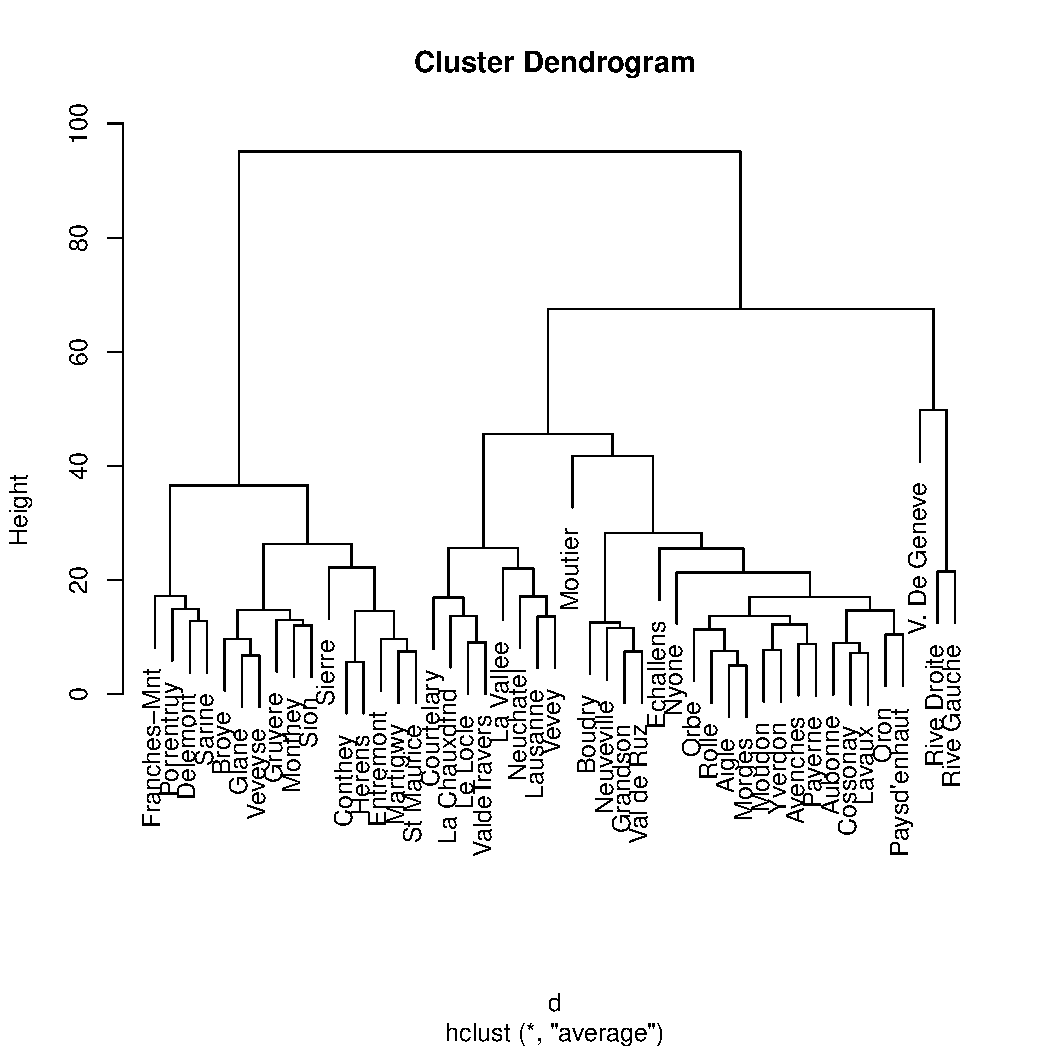
\includegraphics[width=\maxwidth]{figure/unnamed-chunk-3-1} 
\end{knitrout}

\end{document}
